\documentclass[a4paper]{article}

\usepackage{physics,physicsplus}
\newcommand{\note}[1]{{\bf #1}}

\title{Optimal future waveform placement guided by Gaussian processes}
\author{Daniel Williams}

\begin{document}\maketitle


The detection of gravitational wave signals in data collected by
facilities such as the Advanced LIGO detectors in the USA rely on the
comparison of noisy data with pre-determined models of the signals
being searched for. In order to increase the efficiency of this
process it is desirable to have access to a wide variety of models in
order to conduct this process, known as matched filtering, through a
large volume of the parameter space for a physical process which
generates gravitational waves, for example, a binary black hole
coalescence (BBH) event.

Models for these events must be produced by computationally expensive
numerical relativity simulations, and as a result of this expense
determining the most efficient exploration of the entire BBH parameter
space is desirable. We present a method, using Gaussian processes, to
determine the optimal placement of future simulations in the BBH
parameter space, given a pre-existing catalogue of waveforms. We
therefore intend to provide a principled method for deciding how to
extend any pre-existing waveform catalogue.

\section{A Gaussian process surrogate}
\label{sec:surrogate}

In order to determine the locations of parameter space which are most
in need of a future simulation, we require some means to determine the
areas of parameter space which \emph{are} well explained by the
current catalogue. To do this we trained a Gaussian process on the
time-domain waveforms from a catalogue of BBH simulations (Georgia
Tech waveform catalogue), using the squared-exponential covariance
function, summing over $a, b$, 
\begin{equation}
  \label{eq:squaredexp}
  k(\vec{x}_i, \vec{x}_j) = \exp( - \lambda_{ab} \frac{1}{2} (\vec{x}_i - \vec{x}_j)^a (\vec{x}_i, \vec{x}_j)^b )
\end{equation}
where $\lambda_{a,b}$ is a metric representing the scale-lengths of
each dimension of the parameter space, and the various $x_i \in X$ are the
coordinates of the training-points in parameter space.

The distribution of training points is displayed in figure \ref{fig:parameterspace}.

\begin{figure*}
  \centering
  \includegraphics[width=\textwidth]{parameters.pdf}
  \caption{The distribution of training points within the numerical relativity BBH parameter space.}
  \label{fig:parameterspace}
\end{figure*}

The values for the elements $\lambda_{ab}$ were determined by finding
the values of $\lambda_{ab}$ which optimise the marginalised
likelihood (the evidence) of the Gaussian process trained off the data
$X$, that is, by finding the $\lambda_{ab}$ such that the quantity
\begin{equation}
  \label{eq:evidence}
  \log p(\vec{y} | X, \lambda_{ab}) = - \frac{1}{2} \vec{y}^T K_y^{-1} \vec{y} - \frac{1}{2} \log|K_y| - \frac{n}{2} \log 2 \pi
\end{equation}
is maximised.


The output of a Gaussian process trained using the parameter-space
training-data $X$, and the corresponding strain values, $y_i \in Y$ is
then capable of interpolating waveform outputs at parameter-space
coordinates which do not exist in the original training set. The full
output of the Gaussian process is not a single interpolated function,
however, but a distribution of plausible functions, and this provides
a measure of the uncertainty in the interpolated function.

The magnitude of this error provides a means of detecting regions of
the parameter-space which are poorly understood, and regions of high
uncertainty should then be targeted for future simulations in order to
improve the validity of the surrogate function across the entire
parameter space. The values of $\lambda_{ab}$ provide an optimal
spacing for these new waveforms, which should be sampled at intervals
of $\log(\lambda_{ab})$ in regions with high uncertainty or regions
outwith the parameter-space region defined by the original training
data. Figure \ref{fig:spacing} shows an 8-dimensional slice in the
parameter space of the BBH waveforms from a Gaussian process trained
off ten waveforms. We can see that even with a small number of
waveforms it is possible to provide some estimate of the correct grid
sampling required to complete the model.

In order to demonstrate that the parameter spacing is reasonably
independent of the number of waveforms used in training the GP the
model was generated with a differing number of training waveforms, and
trained. The scale length for each parameter is found to be
consistently similar, as can be seen in figure

\begin{figure}
  \centering
  \includegraphics{convergence.png}
  \caption{The scale-lengths of the trained Gaussian process given 10, 29, 72, and 164 waveforms.}
  \label{fig:convergence}
\end{figure}

% \note{We need to
%   demonstrate that using so few waveforms is legitimate. Would
%   probably be sensible to replace this plot with the full catalogue
%   plot once it's finished, and then to include a plot showing
%   grid-spacing against the number of waveforms used for training, and
%   show that the answer converges.}

\begin{figure*}
  \centering
  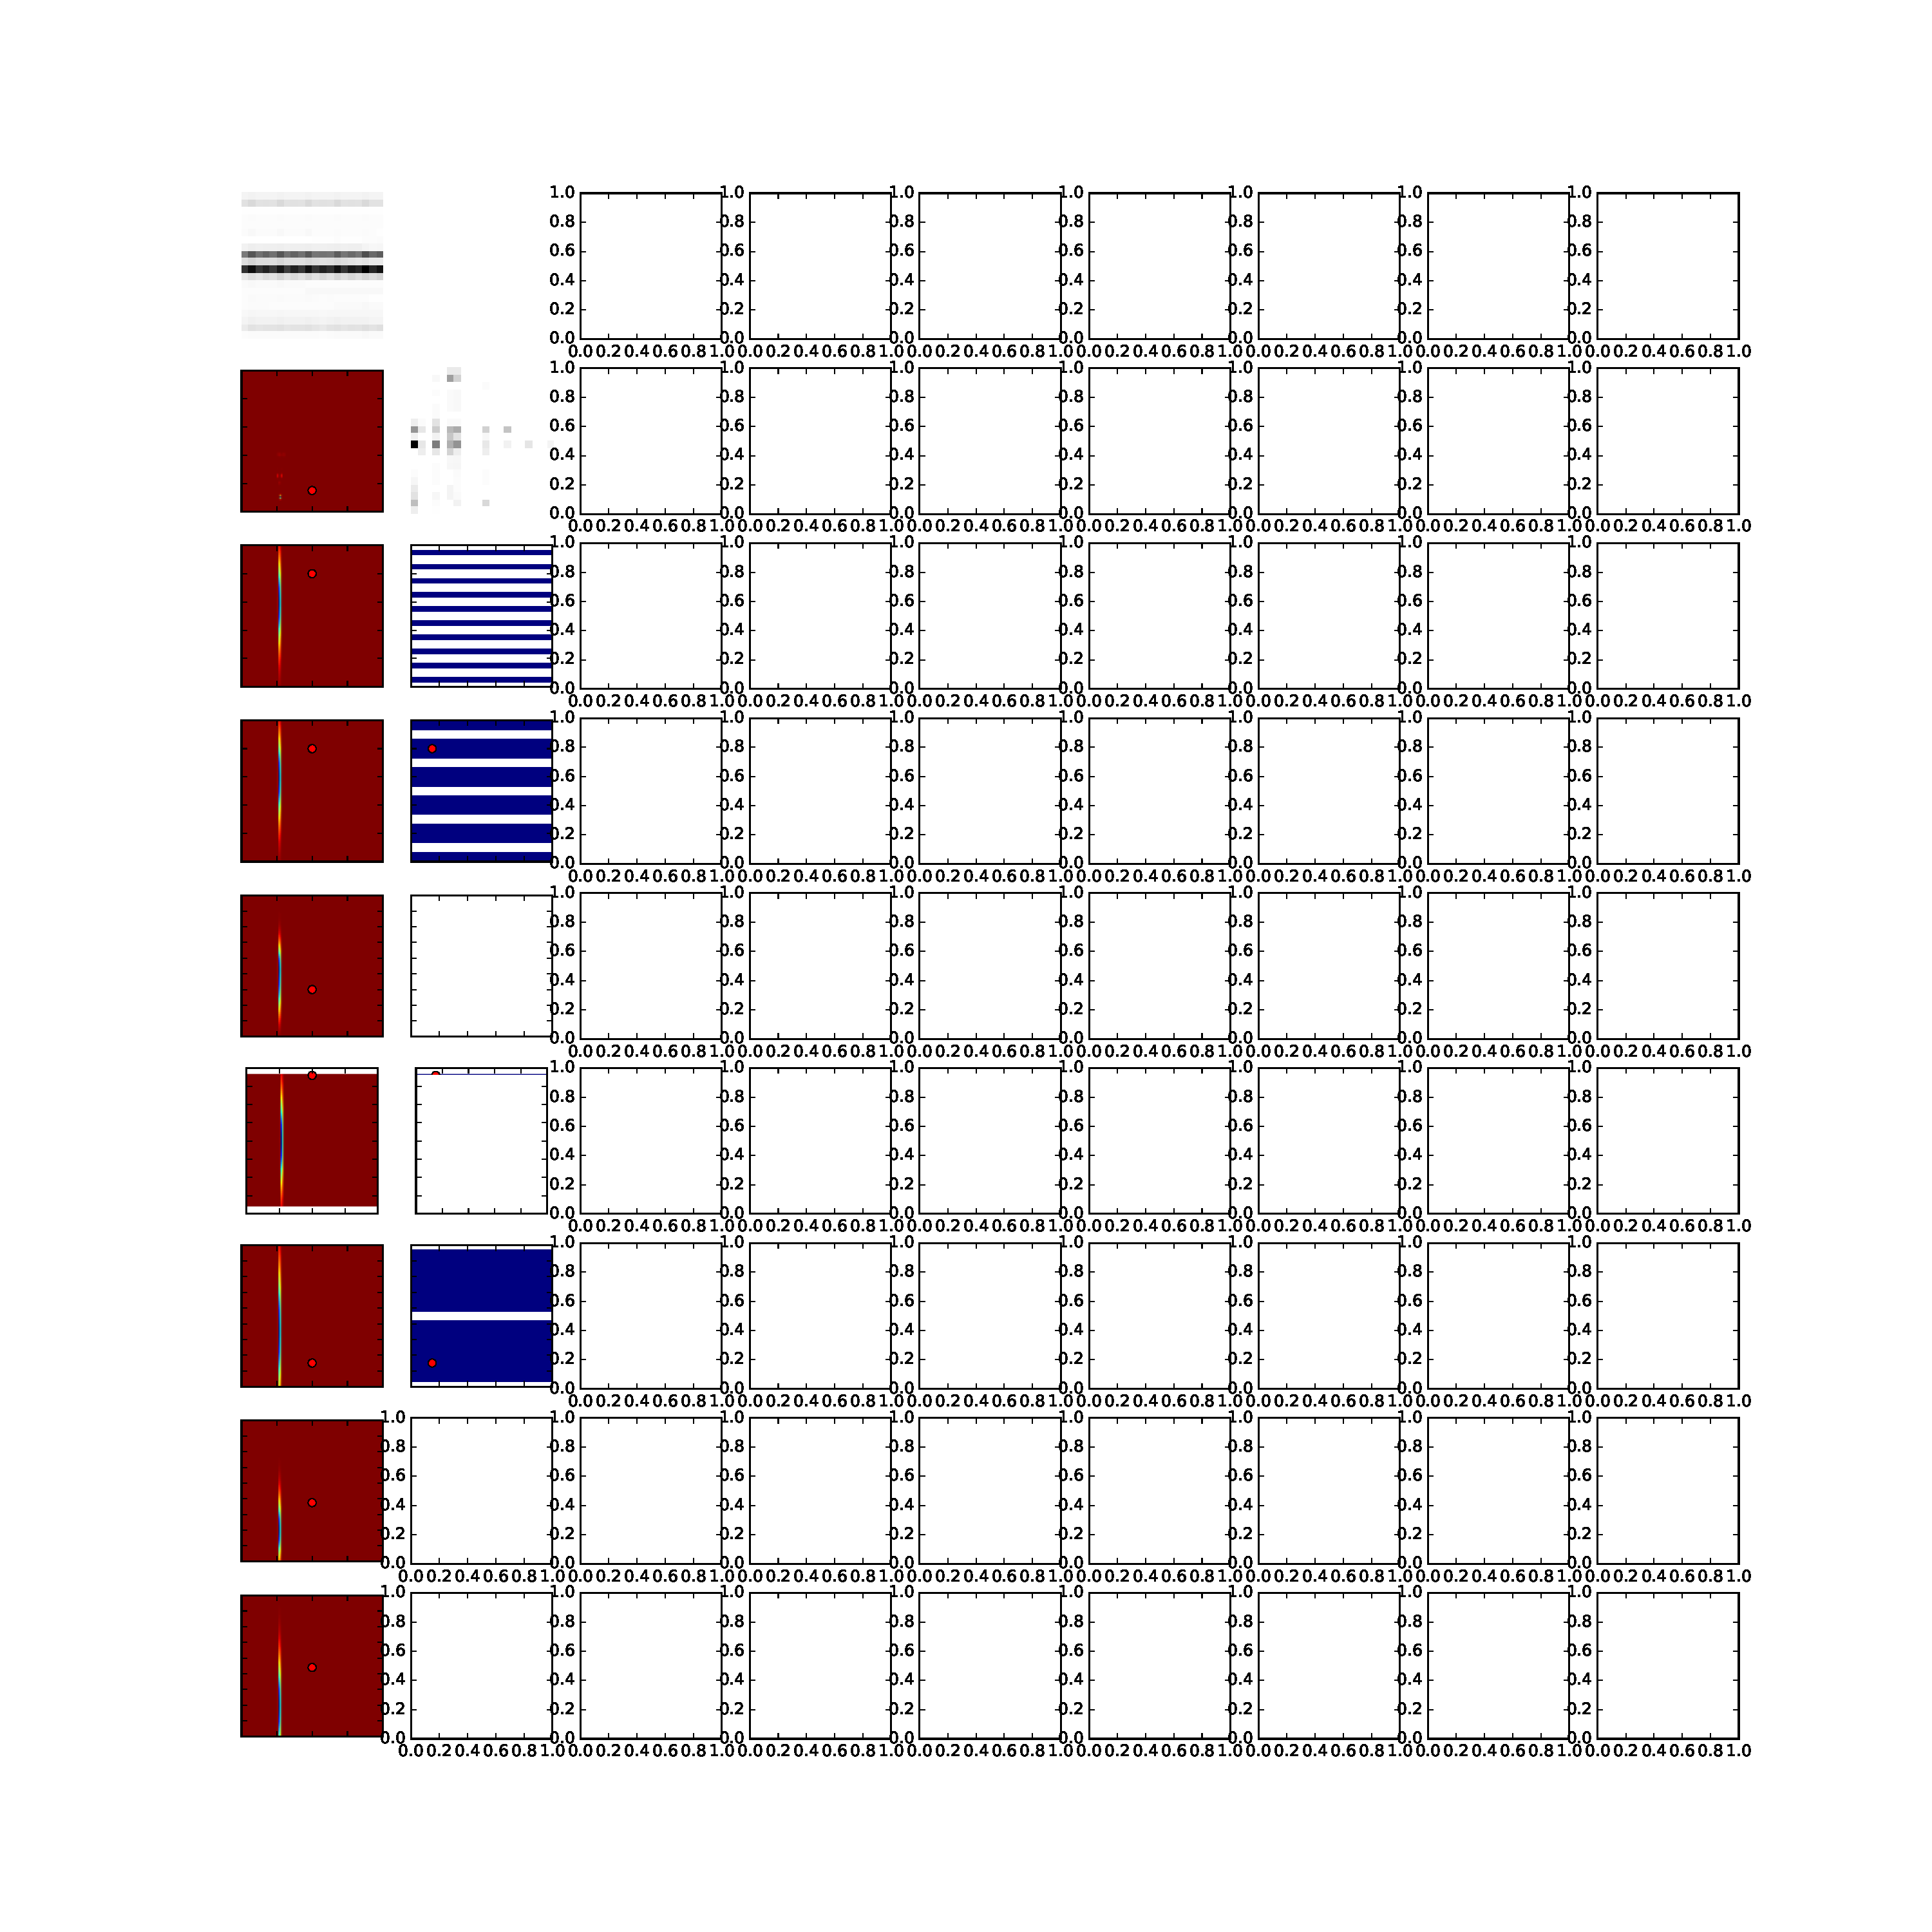
\includegraphics[width=\textwidth]{spacings.pdf}
  \caption{A corner plot of a `hyperslice' the parameter space of the numerical relativity waveforms centred on (0,  1.5,    0.8,    0.8,   60. ,  180. ,   30. ,   75. ,   22. ), showing the variation in the magntiude of the Gaussian process uncertainty over the parameter space in the colorplot, and the optimal spacing as implied by the width of the covariance function. The plots above each column are designed to provide a guide to the density of samples throughout the parameter space in that dimension, while the red point represents the point of intersection of the various planes. }
  \label{fig:spacing}
\end{figure*}

\section{Setting Priorities}
\label{sec:priorities}

Having established the optimal spacing of future waveforms we must
then turn to the question of the optimal order in which they should be
created. Sampling the entire parameter space at the suggested density
would require in excess of 250,000 waveforms, which is an unachievably
large quantity of data.

In other fields which exploit Gaussian processes the choice of future
sample locations can be made usign techniques from Bayesian
optimisation. In these fields the Gaussian process is often emulating
the behaviour of a complicated function surface, and the desired
outcome is finding an optimum on this surface, for example, if a GP is
used to model the distribution of pollutants in a lake, with the aim
of identifying the source of the pollution we may want to find the
region with the maximum amount of pollutant. 

In the case of gravitational waveform modelling we are not terribly
interested in the location of the function's maximum, but instead have
the objective of achieving the greatest quantity of knowledge possible
in the shortest possible period of time (or equivalently, with the
smallest number of function evaluations). In this case the choice of
future samples might be made to minimise the mean-squared error of the
model.

The mean squared error can be calculated using testing data,
$(x^*, y^*)_i$, as
\begin{equation}
  \label{eq:mse}
  {\rm MSE} = \sum_i (y_i^* - f(x_i^*))^2,
\end{equation}
but this requires setting-aside a fraction of our available training
data. Given the small number of samples available, and the large
volume of the parameter space this is likely to have a considerable
impact on the predictive capability of the model. Other options are
available, such as comparing the output to an analytical model, for
example \texttt{IMRPhenomP}, but these approaches suffer from the
incomplete understanding of the uncertainties in these models.

One possible approach is to use a force-based layout of the future
sampling points. By evaluating a force from each of the existing
training points over the parameter space it should be possible to
identify the areas of greatest `emptiness' within the parameter
space. We can then quantise this space using the sampling intervals
derived from the Gaussian process, and place a sample on the grid
point closest to the equilibrium point for the new sample.
\end{document}
